% Options for packages loaded elsewhere
\PassOptionsToPackage{unicode}{hyperref}
\PassOptionsToPackage{hyphens}{url}
%
\documentclass[
]{article}
\usepackage{amsmath,amssymb}
\usepackage{iftex}
\ifPDFTeX
  \usepackage[T1]{fontenc}
  \usepackage[utf8]{inputenc}
  \usepackage{textcomp} % provide euro and other symbols
\else % if luatex or xetex
  \usepackage{unicode-math} % this also loads fontspec
  \defaultfontfeatures{Scale=MatchLowercase}
  \defaultfontfeatures[\rmfamily]{Ligatures=TeX,Scale=1}
\fi
\usepackage{lmodern}
\ifPDFTeX\else
  % xetex/luatex font selection
\fi
% Use upquote if available, for straight quotes in verbatim environments
\IfFileExists{upquote.sty}{\usepackage{upquote}}{}
\IfFileExists{microtype.sty}{% use microtype if available
  \usepackage[]{microtype}
  \UseMicrotypeSet[protrusion]{basicmath} % disable protrusion for tt fonts
}{}
\makeatletter
\@ifundefined{KOMAClassName}{% if non-KOMA class
  \IfFileExists{parskip.sty}{%
    \usepackage{parskip}
  }{% else
    \setlength{\parindent}{0pt}
    \setlength{\parskip}{6pt plus 2pt minus 1pt}}
}{% if KOMA class
  \KOMAoptions{parskip=half}}
\makeatother
\usepackage{xcolor}
\usepackage[margin=1in]{geometry}
\usepackage{graphicx}
\makeatletter
\def\maxwidth{\ifdim\Gin@nat@width>\linewidth\linewidth\else\Gin@nat@width\fi}
\def\maxheight{\ifdim\Gin@nat@height>\textheight\textheight\else\Gin@nat@height\fi}
\makeatother
% Scale images if necessary, so that they will not overflow the page
% margins by default, and it is still possible to overwrite the defaults
% using explicit options in \includegraphics[width, height, ...]{}
\setkeys{Gin}{width=\maxwidth,height=\maxheight,keepaspectratio}
% Set default figure placement to htbp
\makeatletter
\def\fps@figure{htbp}
\makeatother
\setlength{\emergencystretch}{3em} % prevent overfull lines
\providecommand{\tightlist}{%
  \setlength{\itemsep}{0pt}\setlength{\parskip}{0pt}}
\setcounter{secnumdepth}{-\maxdimen} % remove section numbering
\usepackage[utf8]{inputenc}
\usepackage{comment}
\usepackage{todonotes}
\usepackage{amsmath}
\usepackage[ backend=biber, sorting=none, style=authoryear-comp, ]{biblatex}
\usepackage{caption}
\usepackage{adjustbox}
\usepackage{array}
\usepackage{xcolor}
\usepackage{subcaption}
\usepackage{parskip}
\usepackage{graphicx}
\graphicspath{{./images/}}
\usepackage{tikz}
\usetikzlibrary{shapes.geometric, fit, matrix, positioning}
\tikzset{>=latex}
\ifLuaTeX
  \usepackage{selnolig}  % disable illegal ligatures
\fi
\usepackage{bookmark}
\IfFileExists{xurl.sty}{\usepackage{xurl}}{} % add URL line breaks if available
\urlstyle{same}
\hypersetup{
  hidelinks,
  pdfcreator={LaTeX via pandoc}}

\author{}
\date{\vspace{-2.5em}}

\begin{document}

\begin{figure}[h]
\centering
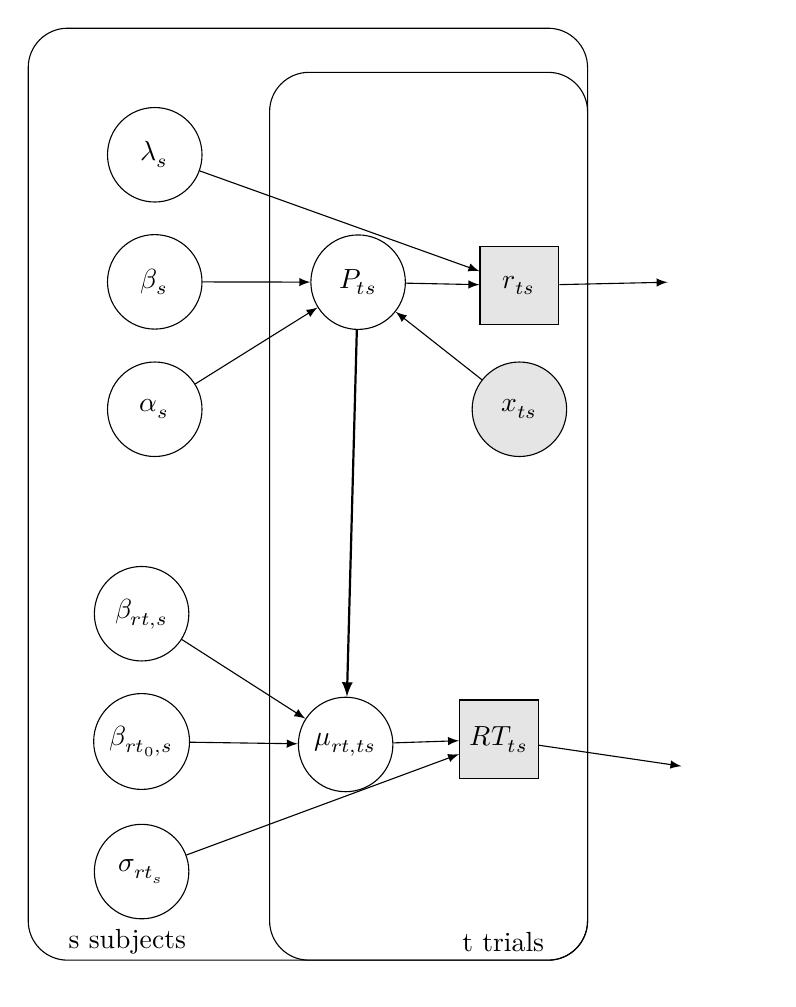
\begin{tikzpicture}
    % Define node styles
    \tikzstyle{circ} = [circle, draw, minimum size=1.2cm]
    \tikzstyle{square} = [rectangle, draw, minimum size=1cm, fill=gray!20]

    % First matrix (m1)
    \matrix (m1) [
        ampersand replacement=\&,
        matrix of math nodes,
        nodes in empty cells,
        column sep=.3cm,
        row sep=0.4cm
    ]
    {
        \&  \& \& \& \&  \& \\
        |[circ]| \lambda_{s} \& \& \& \& \&  \&\\
        |[circ]| \beta_{s} \&  \& \& |[circ]| P_{ts} \& \& |[square]| r_{ts} \\
        |[circ]| \alpha_{s} \&  \& \&   \& \& |[circ, fill=gray!20]| x_{ts}\\
    };

    % Arrows in the first matrix
    \draw[->] (m1-2-1) to (m1-3-6);
    \draw[->] (m1-3-1) to (m1-3-4);
    \draw[->] (m1-4-1) to (m1-3-4);
    \draw[->] (m1-3-4) to (m1-3-6);
    \draw[->] (m1-4-6) to (m1-3-4);

    % Second matrix (m2)
    \matrix (m2) [
        ampersand replacement=\&,
        matrix of math nodes,
        nodes in empty cells,
        column sep=.3cm,
        row sep=0.4cm,
        below=0.5cm of m1
    ]
    {
        \&  \& \& \& \&  \&  \& \\
        |[circ]| \beta_{rt,s}\&  \&  \& \& \&   \\
        |[circ]| \beta_{rt_0,s}\& \& \& |[circ]| \mu_{rt,ts}\&  \& |[square]| RT_{ts}\\
        |[circ]| \sigma_{rt_s}\&  \& \& \& \&  \&\\
        \&  \& \& \& \&  \&\\
    };

    % Arrows in the second matrix
    \draw[->] (m2-2-1) to (m2-3-4);
    \draw[->] (m2-3-1) to (m2-3-4);
    \draw[->] (m2-3-4) to (m2-3-6);
    \draw[->] (m2-4-1) to (m2-3-6);
    
    % Arrow between first matrix (m1) and second matrix (m2)
    \draw[->, thick] (m1-3-4) -- (m2-3-4);

  
    % Combined trial-level box
    \pgfsetcornersarced{\pgfpoint{5mm}{5mm}}
    \node[draw=black, fit=(m1-2-4) (m2-4-6), inner sep=10mm] {}; % subject-level box for both plates

    % Combined subject-level box
    \pgfsetcornersarced{\pgfpoint{5mm}{5mm}}
    \node[draw=black, fit=(m1-2-1) (m2-4-6), inner sep=10mm] {}; % trial-level box for both plates
    
    \node[rotate=0, anchor=west] at (-3.8,-8.7) {s subjects};
    \node[rotate=0, anchor=west] at (1.2,-8.7) {t trials};
    
    
        % New matrix/vector to the right of m1 (o1)
    \matrix (o1) [
        ampersand replacement=\&,
        matrix of math nodes,
        nodes in empty cells,
        column sep=.5cm,
        row sep=0.4cm,
        right=0.5cm of m1
    ]
    {
        \& \\
        \& \\
        \& \\
        \& \\
    };

    % New matrix/vector to the right of m2 (o2)
    \matrix (o2) [
        ampersand replacement=\&,
        matrix of math nodes,
        nodes in empty cells,
        column sep=.5cm,
        row sep=0.4cm,
        right=0.5cm of m2
    ]
    {
        \& \\
        \& \\
        \& \\
        \& \\
    };

    % Arrows to the new matrices
    \draw[->] (m1-3-6) -- (o1-3-1); % From r_{ts} to o1
    \draw[->] (m2-3-6) -- (o2-3-1); % From RT_{ts} to o2
    

\end{tikzpicture}
\caption{Simplified Plate Notation without Non-Decision-Time}
\label{fig:Plate Notation}
\end{figure}


\[
\Phi(x_{ts}, \alpha_{s}, \beta_{s}) = 
0.5+0.5\cdot erf\left(\frac{x_{ts}-\alpha_{s}}{\beta_{s} \cdot \sqrt{2}}\right)
\]

\[
P(x_{ts}, \lambda_{s}, \alpha_{s}, \beta_{s}) = \lambda_{s} + (1 - 2 \lambda_{s}) \cdot \Phi(x_{ts}, \alpha_{s}, \beta_{s})
\]


\[
\mu_{rt,ts} = \beta_{rt_0,s} + \beta_{rt,s} * P(x_{ts}, \lambda_{s}, \alpha_{s}, \beta_{s}) * (1 - P(x_{ts}, \lambda_{s}, \alpha_{s}, \beta_{s}))
\]

\[
RT_{ts} \sim LogNormal(\mu_{rt,ts},\sigma_{rt_s})
\]

\[
r_{ts} \sim Bern(P(x_{ts}, \lambda_{s}, \alpha_{s}, \beta_{s}))
\]


\end{document}
